%% Template baseado no do Prof. Arnaldo Mandel
%% Veja https://www.ime.usp.br/~am/414/listas/index.html

\documentclass[12pt]{article}

%% Escrevendo em português:

%\usepackage[brazilian]{babel}
\usepackage[utf8]{inputenc}
%\usepackage{textcomp}
\usepackage[T1]{fontenc}
\usepackage{lmodern}
%----------------------------

\setlength{\topmargin}{-.5in}
\setlength{\textheight}{9in}
\setlength{\textwidth}{6.3in}
\setlength{\oddsidemargin}{-.125in}
\setlength{\evensidemargin}{-.125in}

\usepackage[usestackEOL]{stackengine}
\usepackage{xspace}
\usepackage{pifont}
\usepackage{amsmath}
\usepackage{amsfonts}
\usepackage[dvipsnames]{xcolor}
\usepackage{fancybox}
\usepackage{amsthm}
\usepackage{listings}
\usepackage{hyperref}
\usepackage{todonotes}

\usepackage{MnSymbol,wasysym}
\usepackage{marvosym}

\pagestyle{empty}

\definecolor{darkgreen}{RGB}{0, 133, 117}
\definecolor{yelloworange}{HTML}{FAA21A}

\newcommand{\N}{{\tt I\kern-.2em N \relax}}      % N        |N
\def\pule{\vspace{0.2cm}}
\def\pulao{\vspace{0.5cm}}
\def\pulaozao{\vspace{1cm}}
\def\ni{\noindent}

\newcommand{\Si}{\ensuremath{\Sigma}\xspace}
\newcommand{\Sis}{\ensuremath{\Sigma^*}\xspace}
\newcommand{\Ga}{\ensuremath{\Gamma}\xspace}
\newcommand{\Gas}{\ensuremath{\Gamma^*}\xspace}
\newcommand{\serio}{\ding{98}\xspace}
\newcommand{\LP}{L\&P\xspace}
\newcommand{\conj}[2]{\ensuremath{\{#1\,|\;#2\}}}
\DeclareMathOperator{\Ima}{Im}
\newcommand{\ssq}{\ensuremath{\subseteq}\xspace}
\newcommand{\union}{\mathop{\bigcup}\displaylimits}
\newcommand{\Rfield}[1]{\ensuremath{\mathbb{R}^{#1}}\xspace}
\newcommand{\del}{\ensuremath{\text{d}}\xspace}
\newcommand{\expct}[1]{\ensuremath{\langle {#1} \rangle}\xspace}

\begin{document}

\newtheorem{theorem}{Teorema}%[section]
\newtheorem{corollary}{Corolário}[theorem]
\newtheorem{lemma}[theorem]{Lema}

\begin{center}
\Huge \bf
Parallelizing GCC with Threads
\vspace{0.5cm}
\end{center}
\vspace*{\fill}
{
     \centering
     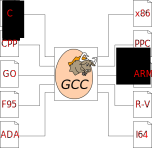
\includegraphics[scale=0.7]{logo.pdf}
    \par
}
\vspace*{\fill}
\normalsize{
\noindent\textcolor{darkgreen}{Giuliano Belinassi} \\
Timezone: GMT$-$3:00 \\
University of São Paulo -- Brazil \\
IRC: giulianob in \#gcc \\
Email: \href{mailto:giuliano.belinassi@usp.br}{\texttt{giuliano.belinassi@usp.br}} \\
Github: \url{https://github.com/giulianobelinassi/} \\
Date: \today
}
\newpage

\begin{section}{About Me}
    Computer Science Bachelor (University of São Paulo), 
    currently pursuing a Masters Degree in Computer Science at the same
    institution. I've always been fascinated by topics such as
    High-Performance Computing and Code Optimization, having worked with
    a parallel implementation of a Boundary Elements Method software in GPU.
    I am currently conducting research on compiler parallelization and,
    therefore, a GSoC internship working with the GNU
    Compiler Collection (GCC) on a related topic is an excellent opportunity
    for me to become more involved with the Free Software community.

    \textbf{Skills}: Strong knowledge in C, Concurrency, Shared Memory Parallelism, command line utilities (grep, sed\dots) and other typical programming tools.
\end{section}

\begin{subsection}{Contributions to GCC}

I've submitted some patches, mainly adding inline optimizations to
trigonometric functions. This kind of patch requires exaustive testing to guarantee
that the optimization does not yield severely incorrect results. This work
resulted in a blog post\footnote{\url{https://flusp.ime.usp.br/gcc/2019/03/26/making-gcc-optimize-some-trigonometric-functions/}} 
about the patch \textit{Optimize sin(arctan(x))}.
I did this blog post both to register how to add this kind of optimization
and also to encourage newcomers to contribute to GCC.

\begin{table}[!htbp]
\centering
\begin{tabular}{|l|l|}
\hline
Name                                                                                      & Status   \\ \hline
    \href{https://patchwork.ozlabs.org/patch/981596/}{Optimize $\sin (\arctan (x))$}      & \color{darkgreen}{\texttt{Accepted}} \\ \hline
    \href{https://patchwork.ozlabs.org/patch/1003988/}{Optimize $\sinh (\text{arctanh} (x))$}   & \color{darkgreen}{\texttt{Accepted}} \\ \hline
    \href{https://patchwork.ozlabs.org/patch/961362/}{Fix typo 'exapnded'}                & \color{darkgreen}{\texttt{Accepted}} \\ \hline
    \href{https://en.wikibooks.org/wiki/LaTeX/Hyperlinks}{Split 'opt and gen' variable}   & \color{yelloworange}{\texttt{Working on}} \\ \hline
    \href{https://patchwork.ozlabs.org/patch/1023211/}{Update $\sin (\arctan (x))$ test}  & \color{yelloworange}{\texttt{Waiting Stage1}} \\ \hline
    \href{https://patchwork.ozlabs.org/patch/1046302/}{Fix PR89437}                           & Wilco Dijkstra version accepted \\ \hline
\end{tabular}
\end{table}

\end{subsection}

\begin{section}{Parallelization Project}
While looking for topics in the compiler field that touched subjects that I
am interested for my masters thesis, I found a
parallelization project proposed in GSoC 2018. With this in mind, I started a
discussion in the mailing list to understand what that project is about,
which was parallelizing GCC internals to be able to compile big files
faster\footnote{\url{https://gcc.gnu.org/ml/gcc/2018-11/msg00073.html}}.
As can be seen in the discussion, I started to work on this subject way before
the list of GSoC accepted organizations was made public.

As stated in PR84402\footnote{\url{https://gcc.gnu.org/bugzilla/show\_bug.cgi?id=84402}},
there is a parallelism bottleneck in GCC concerning huge files (with hundreds of
thousands of lines of code). In the course of the discussion,
Bin Cheng\footnote{\url{https://gcc.gnu.org/ml/gcc/2018-12/msg00079.html}}
reported that
he is affected by this issue, stating that parallelizing the
compiler may solve his problem. These discussions demonstrate the
community interest in this project.

\begin{subsection}{Current Status}
In PR84402, Martin Liška posted a graphic showing the existence of a
parallelism bottleneck in GCC compilation due to huge files such as
\texttt{gimple-match.c} in a 128-cores machine that \texttt{make -j128} alone could not alleviate. He also posted an amazing patch to
GNU Make to collect the data and a script to plot the graphic, which I used
to reproduce the same behaviour in a 64-cores machine that is available at
my university.

Unfortunately, I found this approach not easy to replicate, as
it requires compiling and installing a custom version of Make and generates
gigabytes of data which require parsing by a script that often crashes, as
it struggles to generate a very large SVG. With this in mind, I created a set of
tools\footnote{\url{https://github.com/giulianobelinassi/gcc-timer-analysis}}
using a completely distinct approach, which generates less data, is more stable, and
plots better graphics, such as the one in Figure \ref{fig:analysis}.

I also explored the GCC codebase in order to find the performance bottleneck for
such huge files. I compiled GCC with the
\texttt{--disable-checking} and \texttt{-O2} flags, which
give a more performant (but less reliable) compiler and used this version to compile
\texttt{gimple-match.c} (the largest file in GCC). In this context, I found that the method
\texttt{finalize\_compilation\_unit} of
class \texttt{symbol\_table} takes around $50s$ of the compilation time, with the
\texttt{expand\_all\_functions}
routine taking most of it. Therefore, this routine is a strong candidate for parallelization.

Currently, my strategy to parallelize \texttt{expand\_all\_functions} is to
perform the \texttt{GIMPLE} processing step in parallel, as suggested
by Richard Biener\footnote{\url{https://gcc.gnu.org/ml/gcc/2019-03/msg00249.html}}: each
function may be independently processed by the many passes of
\texttt{GIMPLE}.  There is also a pipelined alternative: a distinct
thread is responsible for a given \texttt{GIMPLE} pass and each
function is fed sequentially to each of them. This allows many
functions to be processed simultaneously, each by a different pass.

Furthermore, I am also studying the theoretical background behind \texttt{GIMPLE}
and \texttt{cgraphs}. I have read the \texttt{GIMPLE}
documentation\footnote{\url{https://gcc.gnu.org/onlinedocs/gccint/}} and
I am looking at how \texttt{cgraph} works internally, both in theory and within
GCC.

\end{subsection}

\begin{subsection}{Planned Tasks}

I plan to use the GSoC time to develop the following topics:

\begin{itemize}
 \item{Week [1, 7] -- May 6 to June 21:} \\
Refactor \texttt{cgraph\_node::expand()} and
\texttt{expand\_all\_functions}, splitting \texttt{IPA},
\texttt{GIMPLE} and \texttt{RTL} passes, and some documentation about
the global states of the \texttt{GIMPLE} passes.
 \item{Week 8 -- June 24 to 28:} \textbf{First Evaluation} \\
Deliver a patch with the refactored version of \texttt{cgraph\_node::expand()} and
\texttt{expand\_all\_functions}, and the partial documentation
with regard to \texttt{GIMPLE}.
 \item{Week [9, 11] -- July 1 to 19:} \\
Continue documentating and refactoring the \texttt{GIMPLE} passes, and
prototype a parallelization of \texttt{expand\_all\_functions}.
 \item{Week 12 --- July 22 to 26:} \textbf{Second Evaluation} \\
Attend to Debconf 19 (Curitiba, Brazil). Please let me know
if someone else from GCC will attend. \\
Deliver a
working non-optimized parallel version of \texttt{expand\_all\_functions}
with the point of being correct in a multi-threaded environment.
\item{Week [13, 15] --- July 29 to August 16:} \\
Iteractively improve the current implementation.
\item{Week 16 - August 19:} \textbf{Final evaluation}\\
Optimize the current implementation, so that there is a speedup over
the sequential version when compiling \texttt{gimple-match.c} and reducing the
total compilation time in \texttt{GCC} compilation without bootstrap.
\end{itemize}

\begin{figure}[ht]
 \centering
 \includegraphics[scale=0.6, angle=-90]{out-crop.pdf}
 \caption{Elapsed time analysis in GCC compilation for a 64 cores machine, No bootstrap}
 \label{fig:analysis}
\end{figure}

\end{subsection}

\end{section}
\end{document}
